%% ----------------------------------------------------------------------------
% BIWI SA/MA thesis template
%
% Created 09/29/2006 by Andreas Ess
% Extended 13/02/2009 by Jan Lesniak - jlesniak@vision.ee.ethz.ch
%% ----------------------------------------------------------------------------


\chapter{Introduction}


The task of image segmentation into binary classes is very useful in different cases in biomedical tasks. It can be used for detection of diseases, shape analysis etc. The methods to solve the segmentation problem has evolved among two lines: 1) level of interaction: from semi-interactive to fully automatic, and 2) level of classification: pixels to complete images. Nowadays, with the use of fully-convolutional networks, the segmentation can be obtained for complete image in one forward pass. This helps in using the local as well as contextual information for segmentation. Currently, the benchmark performance in terms of accuracy is achieved by the use of convolutional neural networks (CNN). The neural networks are specialized to learn feature maps from the examples provided and specific to task at hand. These networks require huge amount of training data: images and ground truth i.e. label for each pixel in the input image; to train the network from scratch. In literature, we can find different architectures of neural networks specially designed for task of segmentation, one of the popular architecture is U-Net[cite]. This approach works well for tasks where we can find significant number of images and can train a neural network. However, this poses a difficulty when we are trying to segment objects in microscopic images.

\begin{figure}[h!] \label{fig:3dstack}
 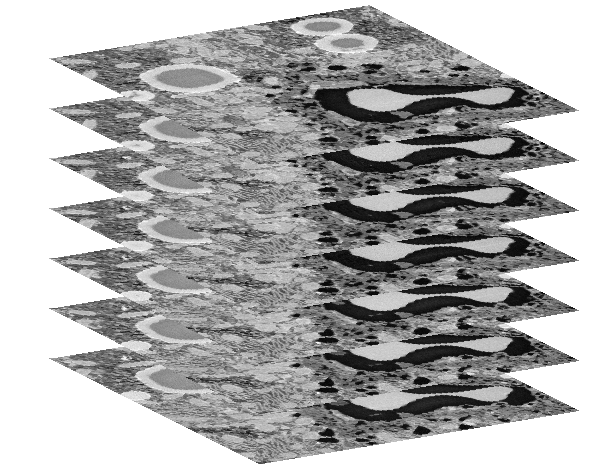
\includegraphics[width=0.8\linewidth]{figures/3d_stack.png}
\caption{A 3D image stack, output from a scanning electron microscope.
The stacks contains 458 2D images with a resolution of 1890x1952 pixel each.}
\end{figure}


\section{Electron Microscopy Images}
The dataset which we are trying to segment are electron microscopic (EM) images of liver tissue. The dataset consists of a 3D stack of 2D slices of liver tissue as shown in figure 1.1. The dataset can be considered as a single 3D stack or multiple 2D slices for our task. We can observe following traits in EM images:
\begin{itemize}
\item High variability between images: The images to be segmented may be entirely different i.e. having fixed objects as in liver tissue or having layers to segments as in neuron tissue. The objects to be segmented may differ completely from being smooth (round vesicles) to branched (neurons). This prohibits use of one dataset to train a network for another dataset and thus, restricting availability of images.
\item High variability between objects to segment: The objects to be segmented vary significanly in shape, size and texture in different images.
\item High variability between goals: Even for a single image, the goal of the segmentation can be totally different. The images annotated for one object can not be used again for training purpose.
\end{itemize}
These characteristics of EM images make it very difficult to fully annotate each object of interest and is extremely time consuming for experts. Here for our task, we are interested to segment vesicles, as shown in figure 1.2. The difficulty to annotate different vesicles of undefined shapes and sizes can be observed in Figure 1.2. To add to this complexity, the experts are uncertain about existence of vesicles in certain part of images and sometimes, even one expert annotates differently at different times. The difference in annotations can be observed for different experts and also for anotations of same image by same expert, as shown in figure 1.3. For example, we can observe differences in rectangular boxes in figure 1.3. This uncertainity has been analyzed in literature and researchers have tried to come up with different methods to get one ground truth mask from these multiple annotations by experts. We can use STAPLE[cite] algorithm or union or majority voting to derive reference mask. The reference mask derived for one slice using STAPLE and union is shown in figure 1.4\par



\begin{figure}[h!] \label{fig:2dslice}
 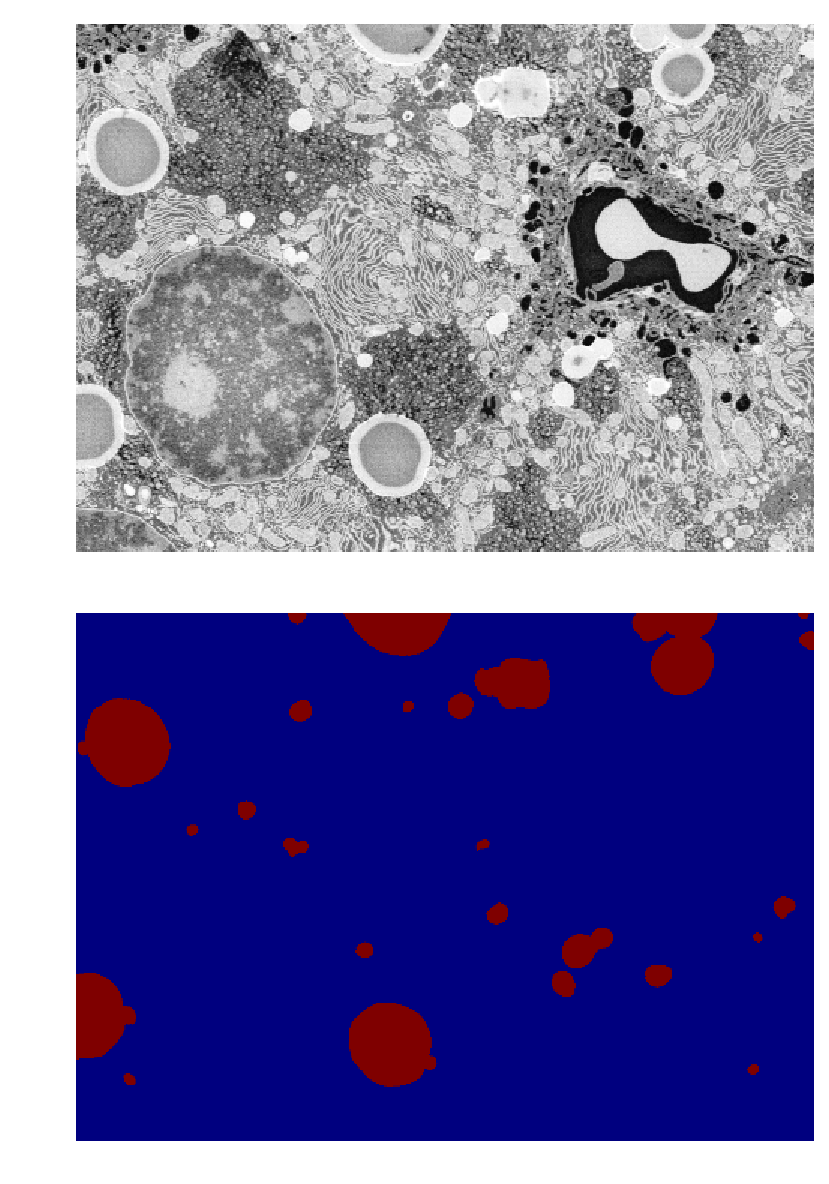
\includegraphics[width=0.7\linewidth]{figures/ex_slice.pdf}
\caption{Cropped part of slice 15 and its ground truth annotation by an expert.}
\end{figure}

\begin{figure}[h!] \label{fig:diffexperts}
 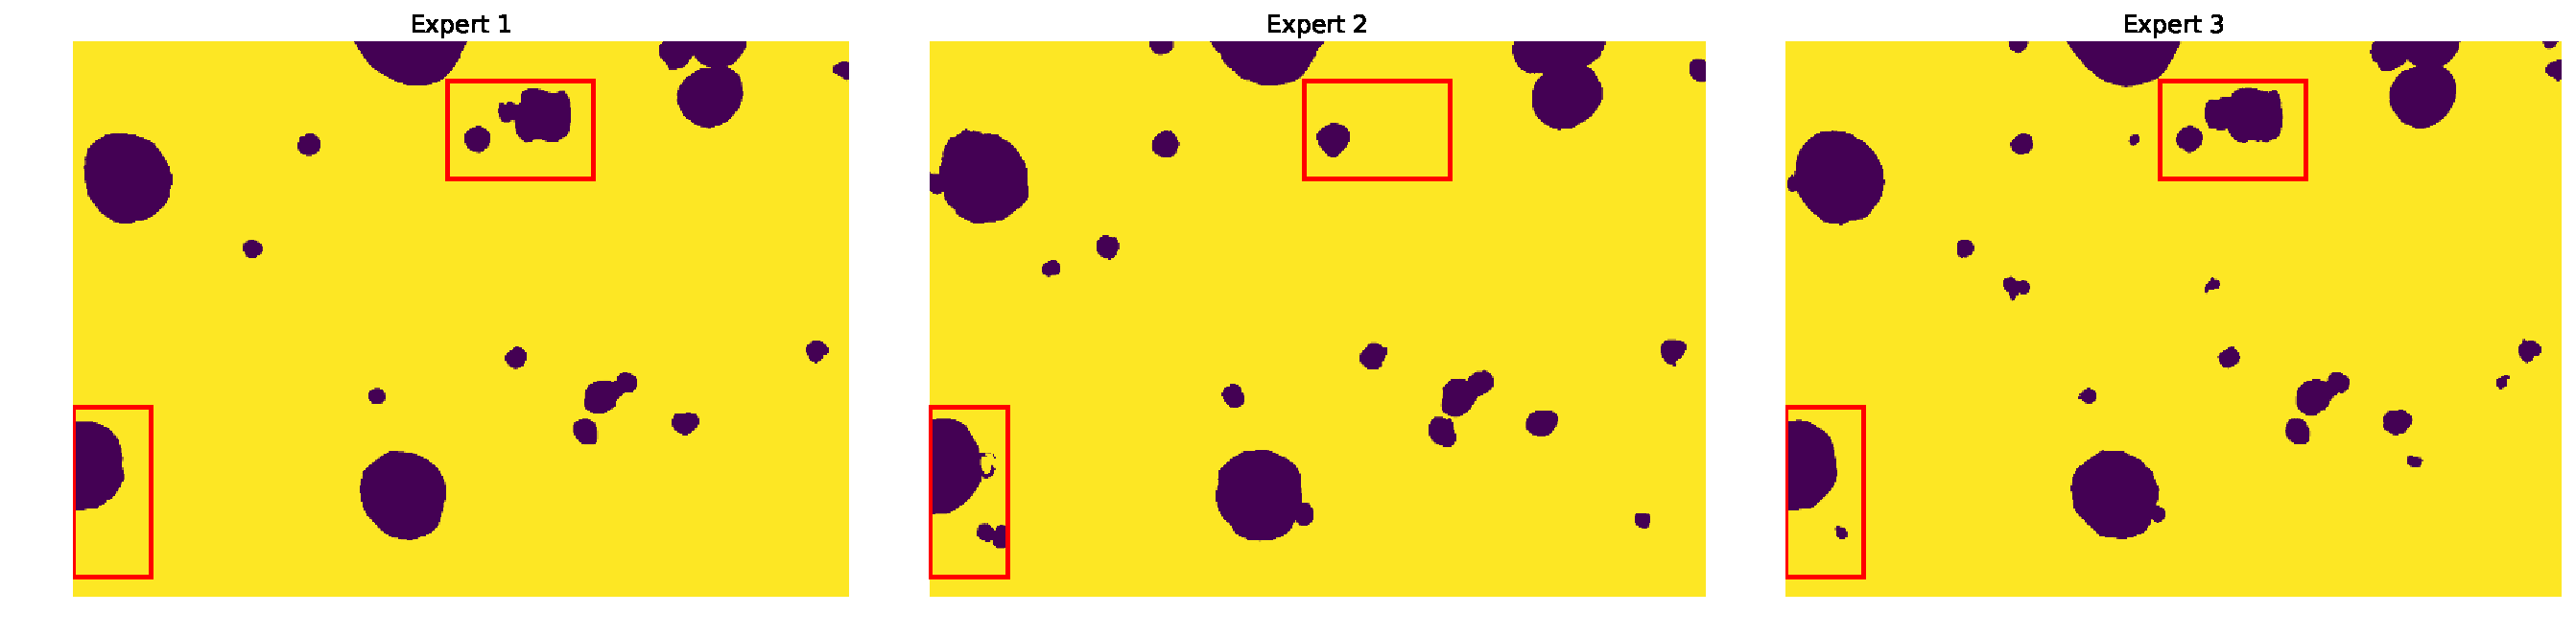
\includegraphics[width=1.0\linewidth]{figures/different_expert.pdf} \\
  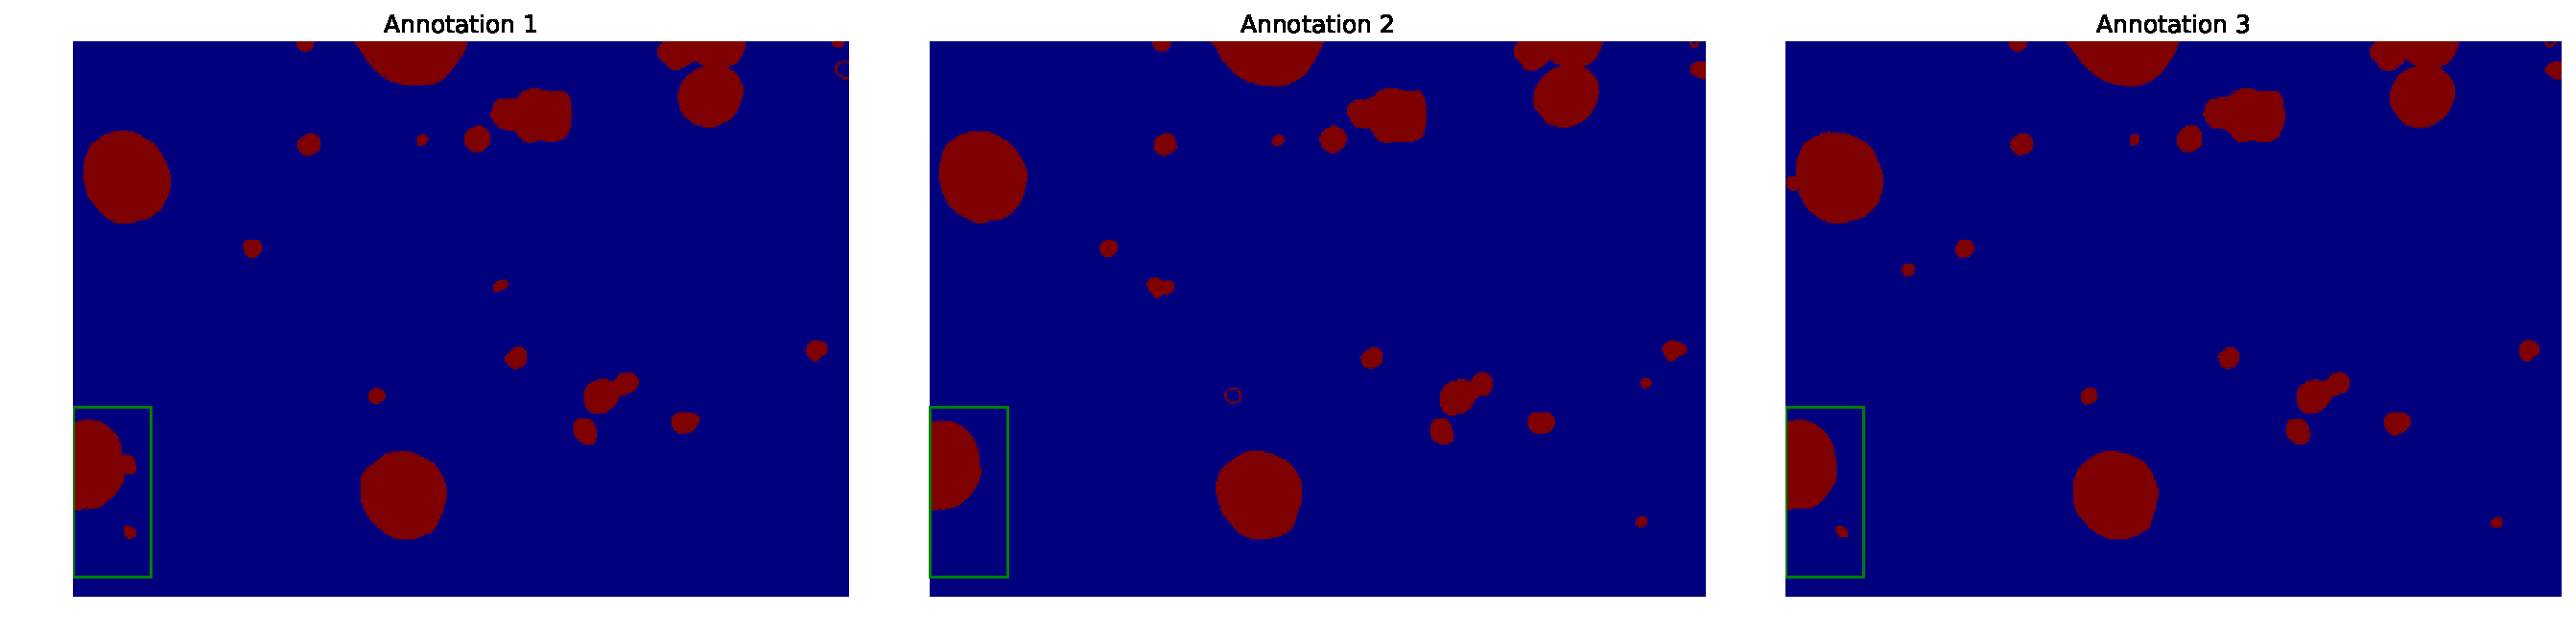
\includegraphics[width=1.0\linewidth]{figures/same_expert.pdf}
\caption{Upper row: Annotation of an slice by different experts. Bottom row: Multiple annotations of an slice by same expert. One example of difference can be observed in bounding boxes.}
\end{figure}

\begin{figure}[] \label{fig:ref}
 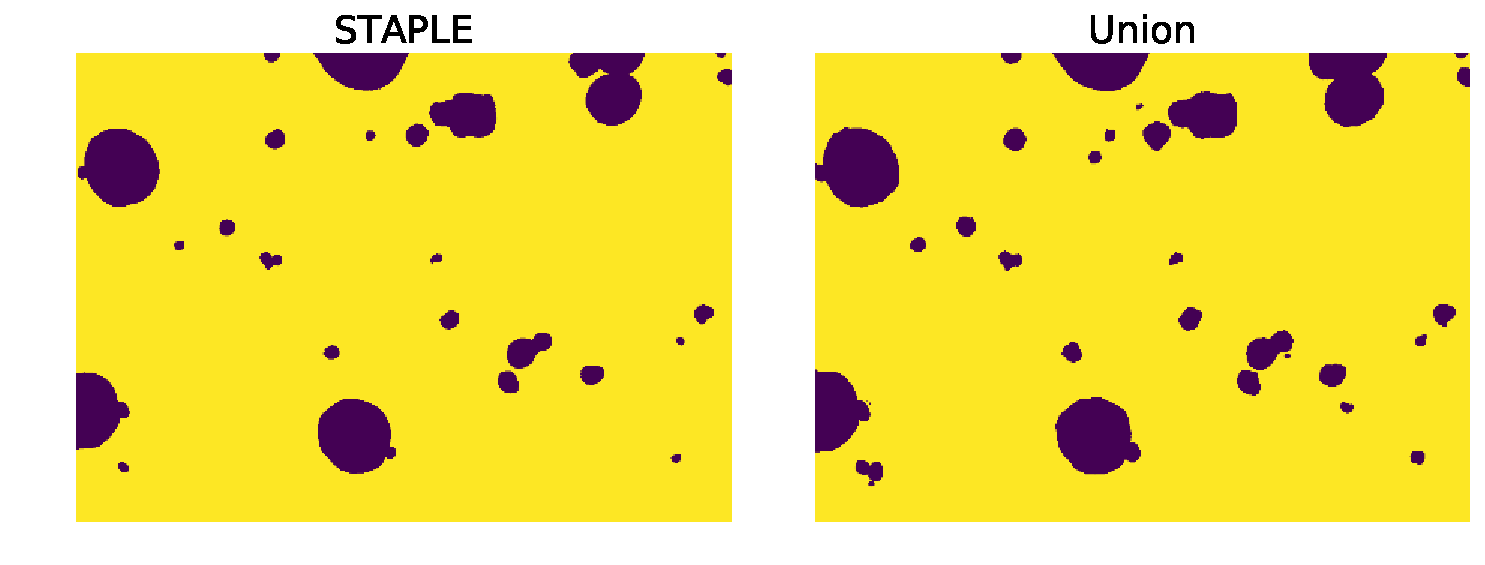
\includegraphics[width=0.7\linewidth]{figures/staple.pdf}
\caption{Grounth truth mask derived from multiple annotaions using 2 different methods}
\end{figure}

\section{Focus of this thesis}
Nowadays, it is common to train deep neural networks (DNN) using transfer learning to compensate for lack of enough data for training. Recently, Shelmar et al[cite] designed a "fully convolutional" network that take input of arbitrary size and produce segmented output for complete image. They adapted contemporary classification networks (AlexNet, the VGG net, and GoogLeNet) into fully convolutional networks and transfer their learned representations by fine-tuning to the segmentation task. Similar to this, we use and finetune network explained in Caelles et al[cite]. This paper tackles the task of \textbf{semi-supervised} video object segmentation, i.e., segment an object in a video, given fully annotated mask of object in the first frame. This task can be considered to be similar to segmenting objectsin 3D stack of slices. We try to finetune the network using fully annotated objects in few slices in the stack. We describe the details and observations in Section 2.

The use of pre-trained networks makes it possible to use DNN even with small amount of training data. But still to train the DNN, we need to provide fully annotated masks for objects of interest for all training images and this comes out to be a tedious and difficult task as explained above. In addition, the presence of multiple objects of different shape and sizes makes it even more diffcult and time consuming. Imagine 1000 cells in a 2D slice and possiblity to manually annotate all these cells of undefined shapes! This provide us with option of annotate few objects and train networks using either cropped images or treating rest of image as background. Or we can use semi-supervised learning using partial annotations. In literature, we can find various methods to use these partial annotation to classify each pixel as foreground or background. For example, Santner[cite] describes use of Random forests (RF) for image segmentation using partial annotations. In this thesis, we try to discover the effect of annotation budget i.e. the number of pixels to annotate and the accuracy achieved. We also try to learn which pixels to annotate to use our annotation budget efficiently. 

These methods only learn pixel level information and are uncertain for maximum of pixels i.e. the probability of foreground learnt is not binary but lies between 0 and 1. In literature, different approaches can be found to use prior information to compensate for data and for the uncertainity of estimators. The most common is to use Conditional random fields (CRFs) or graph cuts to regularize the probability learnt. We solve this problem using a prior in \textbf{Bayesian framework}. Santner[cite] uses weighted total variation as prior and Random forests to learn likelihood. Ranftl[cite] uses CNN to learn unary and edge potential and combine this information to get segmentation mask using graph cuts. For our task, we implement the method described in master thesis of Dominic[cite]. In Dominic[cite], they try to learn likelihood using Random forests and prior as isotropic total variation (TV). They use a non-linear cost function to fomulate likelihood from probabilities learnt from Random forests. This is quite different to common approach of using probabilities directly as likelihood to combine with prior. Majority of researchers using CNN use a linear cost function to implement prior with help of CRFs. In this thesis, we analyze and compare these different cost functions. We try to observe the advantage of using these cost functions in different scenarios. For images as 3D stacks, it is obseved to be a difficult task and computationally efficient to encode 3D information in models as CNN or RF for learning likelihood. Also, it is common practice to use prior information in 2D. Thus, we also try to observe benefits of using 3D isotropic total variation in case of 3D stacks. \par

In summary, we use a Bayesian approach with RF to parametrize likelihood and isotropic TV as prior to predict segmentation mask for a given image. This gives us chance to generate fully annoatated segmentation masks and train CNN to obtain better accuracy. The common problem for use of prior is choice of appropriate scaling to couple likelihood and prior costs. Ranftl[cite] coupled the prior cost function with the likelihood cost function obtained from CNN. They optimized the final loss function to obtain optimal values for network parameters (weigts and biases) and regularization parameter. Riegler[cite] propsed a method to implement TV as specialized layers in CNN and trained the complete model, CNN + TV, together. This motivated us to replace RF with CNN and try to learn pretrained fully convolutional network from partial annotations. We were able to restructure cross-entropy loss to compute loss for partial annotations. \newline
Finally, we also showed advantage of using iterative semi-interactivity for efficient use of annotation budget and also to be able to provide opportunity to experts to improve learning method according to their specific requirements.

\section{Thesis Organization}
The thesis is divided mainly into two sections: segmentation using fully annotated objects and segmentation using partial annotations. The segmentation using full annotations is described in Section 2. The later method is described in Section 3. In section 3.1, we describe improvement in segmentation mask for increased labelling effort. We introduce use of prior and variational methods in section 3.2. In section 3.3, we introduce use CNN to learn from partial annotations. Finally, in section we conclude this thesis and lay out future work that can be done.



